% create a png with latexmk states.tex -shell-escape

% \documentclass[12pt]{article} % use this one for pdf output
\documentclass[preview,border=4mm,convert={density=600,outext=.png}]{standalone} % use this one for png output

\usepackage[english]{babel}
\usepackage[utf8x]{inputenc}
\usepackage{amsmath}
\usepackage{tikz}
\usetikzlibrary{arrows,automata}
\begin{document}

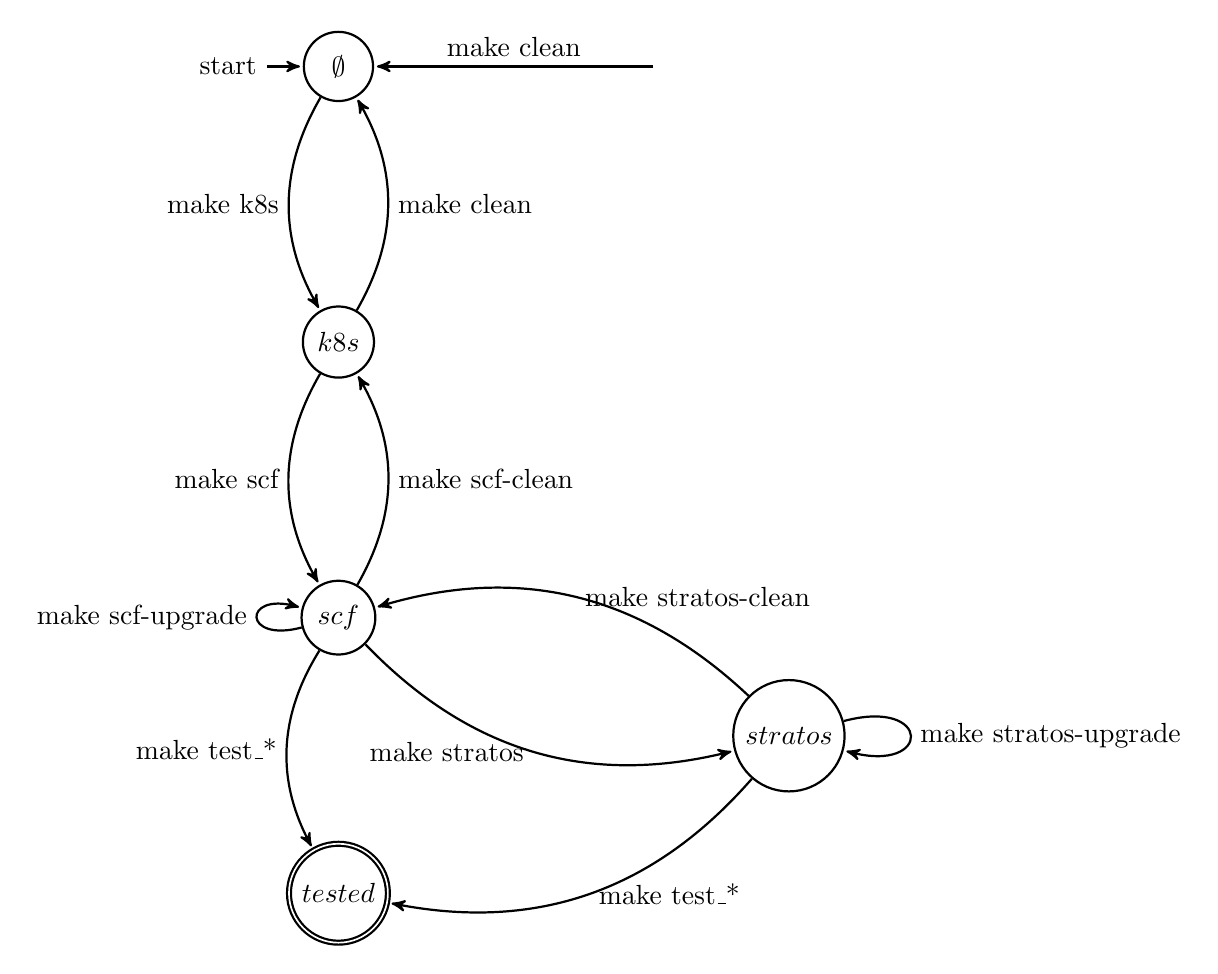
\begin{tikzpicture}[->,>=stealth',shorten >=1pt,auto,node distance=3.5cm,
        scale = 1,transform shape, thick]

  \node[state,initial] (zero) {$\emptyset$};
  \node[state] (k8s) [below of=zero] {$k8s$};
  \node[state] (scf) [below of=k8s] {$scf$};
  \node[state] (stratos) [below of=scf,above=2cm, right=5cm] {$stratos$};
  \node[state,accepting] (tested) [below of=scf] {$tested$};
  \node (all) [right of=zero, right=0.5cm] {};

  \path
        (zero)    edge[bend right, left]   node {make\ k8s} (k8s)
        (k8s)     edge[bend right,right]   node {make\ clean} (zero)
        (all)     edge[above]              node {make\ clean} (zero)
        (k8s)     edge[bend right, left]   node {make\ scf} (scf)
        (scf)     edge[bend right,right]   node {make\ scf-clean} (k8s)
        (scf)     edge[bend right, left]   node {make\ stratos} (stratos)
        (scf)     edge[loop left, left]    node {make\ scf-upgrade} (scf)
        (stratos) edge[bend right,right]   node {make\ stratos-clean} (scf)
        (stratos) edge[loop right, right]  node {make\ stratos-upgrade} (stratos)
        (scf)     edge[bend right, left]   node {make\ test\_*} (tested)
        (stratos) edge[bend left, right]   node {make\ test\_*} (tested);

\end{tikzpicture}
\end{document}